\documentclass{beamer}
\usepackage{pgfpages}
\setbeamertemplate{caption}[numbered]
\setbeamertemplate{caption label separator}{: }
\setbeamercolor{caption name}{fg=normal text.fg}
\beamertemplatenavigationsymbolsempty
% Prevent slide breaks in the middle of a paragraph:
\widowpenalties 1 10000
\raggedbottom
\setbeamertemplate{part page}{
  \centering
  \begin{beamercolorbox}[sep=16pt,center]{part title}
    \usebeamerfont{part title}\insertpart\par
  \end{beamercolorbox}
}
\setbeamertemplate{section page}{
  \centering
  \begin{beamercolorbox}[sep=12pt,center]{part title}
    \usebeamerfont{section title}\insertsection\par
  \end{beamercolorbox}
}
\setbeamertemplate{subsection page}{
  \centering
  \begin{beamercolorbox}[sep=8pt,center]{part title}
    \usebeamerfont{subsection title}\insertsubsection\par
  \end{beamercolorbox}
}
\AtBeginPart{
  \frame{\partpage}
}
\AtBeginSection{
  \ifbibliography
  \else
    \frame{\sectionpage}
  \fi
}
\AtBeginSubsection{
  \frame{\subsectionpage}
}
\usepackage{lmodern}
\usepackage{amssymb,amsmath}
\usepackage{ifxetex,ifluatex}
\ifnum 0\ifxetex 1\fi\ifluatex 1\fi=0 % if pdftex
  \usepackage[T1]{fontenc}
  \usepackage[utf8]{inputenc}
  \usepackage{textcomp} % provides euro and other symbols
\else % if luatex or xelatex
  \usepackage{unicode-math}
  \defaultfontfeatures{Scale=MatchLowercase}
  \defaultfontfeatures[\rmfamily]{Ligatures=TeX,Scale=1}
\fi
% use upquote if available, for straight quotes in verbatim environments
\IfFileExists{upquote.sty}{\usepackage{upquote}}{}
\IfFileExists{microtype.sty}{% use microtype if available
  \usepackage[]{microtype}
  \UseMicrotypeSet[protrusion]{basicmath} % disable protrusion for tt fonts
}{}
\makeatletter
\@ifundefined{KOMAClassName}{% if non-KOMA class
  \IfFileExists{parskip.sty}{%
    \usepackage{parskip}
  }{% else
    \setlength{\parindent}{0pt}
    \setlength{\parskip}{6pt plus 2pt minus 1pt}}
}{% if KOMA class
  \KOMAoptions{parskip=half}}
\makeatother
\usepackage{xcolor}
\IfFileExists{xurl.sty}{\usepackage{xurl}}{} % add URL line breaks if available
\IfFileExists{bookmark.sty}{\usepackage{bookmark}}{\usepackage{hyperref}}
\hypersetup{
  pdftitle={Multivariate fault detection in WWTP},
  pdfauthor={Kathryn B. Newhart},
  pdfborder={0 0 0},
  breaklinks=true}
\urlstyle{same}  % don't use monospace font for urls
\newif\ifbibliography
\usepackage{graphicx,grffile}
\makeatletter
\def\maxwidth{\ifdim\Gin@nat@width>\linewidth\linewidth\else\Gin@nat@width\fi}
\def\maxheight{\ifdim\Gin@nat@height>\textheight\textheight\else\Gin@nat@height\fi}
\makeatother
% Scale images if necessary, so that they will not overflow the page
% margins by default, and it is still possible to overwrite the defaults
% using explicit options in \includegraphics[width, height, ...]{}
\setkeys{Gin}{width=\maxwidth,height=\maxheight,keepaspectratio}
\setlength{\emergencystretch}{3em}  % prevent overfull lines
\providecommand{\tightlist}{%
  \setlength{\itemsep}{0pt}\setlength{\parskip}{0pt}}
\setcounter{secnumdepth}{-2}

% set default figure placement to htbp
\makeatletter
\def\fps@figure{htbp}
\makeatother

%\usepackage{xcolor}
% \usetheme{CambridgeUs}
% =================
% = Define Colors =
% =================
%\definecolor{CSMnavy}{RGB}{0,35,75}
%\definecolor{CSMorange}{RGB}{241,90,42}
%\definecolor{CSMblue}{RGB}{134,157,193}


%\setbeamercolor{frametitle}{blue}
%\setbeamercolor{title}{Blue}

%\setbeamertemplate{navigation symbols}{}
%\setbeamertemplate{footline}[frame number]


\setbeamertemplate{navigation symbols}{}
%\institute{Department of Political Science}
%\titlegraphic{\includegraphics[width=0.3\paperwidth]{\string~/Dropbox/teaching/clemson-academic.png}}
\setbeamertemplate{title page}[empty]

\setbeamerfont{subtitle}{size=\small}

\setbeamercovered{transparent}

\definecolor{clemsonpurple}{HTML}{522D80}
\definecolor{clemsonorange}{HTML}{F66733}

\definecolor{uiucblue}{HTML}{003C7D}
\definecolor{uiucorange}{HTML}{F47F24}

\setbeamercolor{frametitle}{fg=clemsonpurple,bg=white}
\setbeamercolor{title}{fg=clemsonpurple,bg=white}
\setbeamercolor{local structure}{fg=clemsonpurple}
\setbeamercolor{section in toc}{fg=clemsonpurple,bg=white}
% \setbeamercolor{subsection in toc}{fg=clemsonorange,bg=white}
\setbeamercolor{footline}{fg=clemsonpurple!50, bg=white}
\setbeamercolor{item projected}{fg=clemsonpurple,bg=white}
\setbeamertemplate{itemize item}{\color{clemsonpurple}$\bullet$}
\setbeamertemplate{itemize subitem}{\color{clemsonpurple}\scriptsize{$\bullet$}}
\let\Tiny=\tiny

\AtBeginPart{}
\AtBeginSection{}
\AtBeginSubsection{}
\AtBeginSubsubsection{}
\setlength{\emergencystretch}{0em} % prevent overfull lines
\setlength{\parskip}{0pt}

\defbeamertemplate*{footline}{my footline}
{
\ifnum \insertpagenumber=1

\leavevmode%
\hbox{%
\begin{beamercolorbox}[wd=\paperwidth,ht=.80ex,dp=1ex,center]{}%
% empty environment to raise height
\end{beamercolorbox}}%
\vskip0pt%
\else

\hspace*{.5cm}\Tiny{%
\hspace*{50pt} \hfill\insertframenumber/\inserttotalframenumber\hspace*{.00cm} \\ \vspace*{5pt}}%

\fi
}

\title{Multivariate fault detection in WWTP}
\author{Kathryn B. Newhart}
\date{February 13, 2019}
\institute{Colorado School of Mines}

\begin{document}
\frame{\titlepage}

\begin{frame}{Introduction to fault detection}
\protect\hypertarget{introduction-to-fault-detection}{}

\begin{itemize}
\tightlist
\item
  Single variable monitoring is \textbf{traditional approach} in WWTP
\item
  Trend analysis is used, but methods are kept \textbf{private}
\item
  Multivariate statistical process monitoring is \textbf{widespread in
  literature}, but \emph{not in practice}
\end{itemize}

\end{frame}

\begin{frame}{Why use statistical process control?}
\protect\hypertarget{why-use-statistical-process-control}{}

\begin{itemize}
\tightlist
\item
  Statistical Process Control (SPE)
\item
  There is \textbf{inherent variability} in WWTP that cannot be
  accounted for with an empirical model
\item
  Operator-determined setpoints may not be valid for all operating
  conditions, making the system reliant on diligent supervison.
\item
  \textbf{To improve efficiency, need to improve process control}
\end{itemize}

\end{frame}

\begin{frame}{Why use statistical process control?}
\protect\hypertarget{why-use-statistical-process-control-1}{}

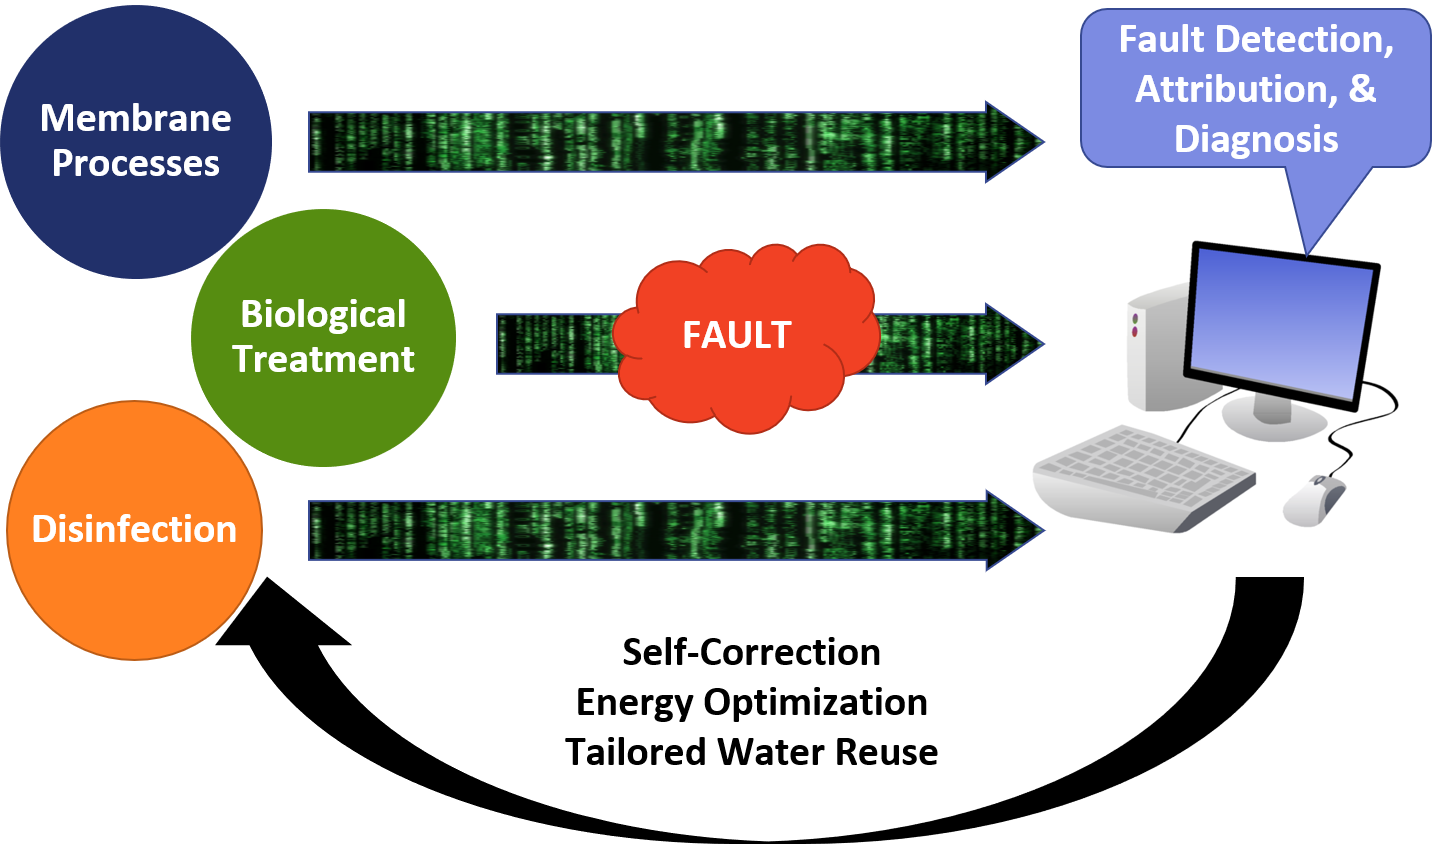
\includegraphics{images/wwtp_data_fault_diagram.png}

\end{frame}

\begin{frame}{Characteristics of big data}
\protect\hypertarget{characteristics-of-big-data}{}

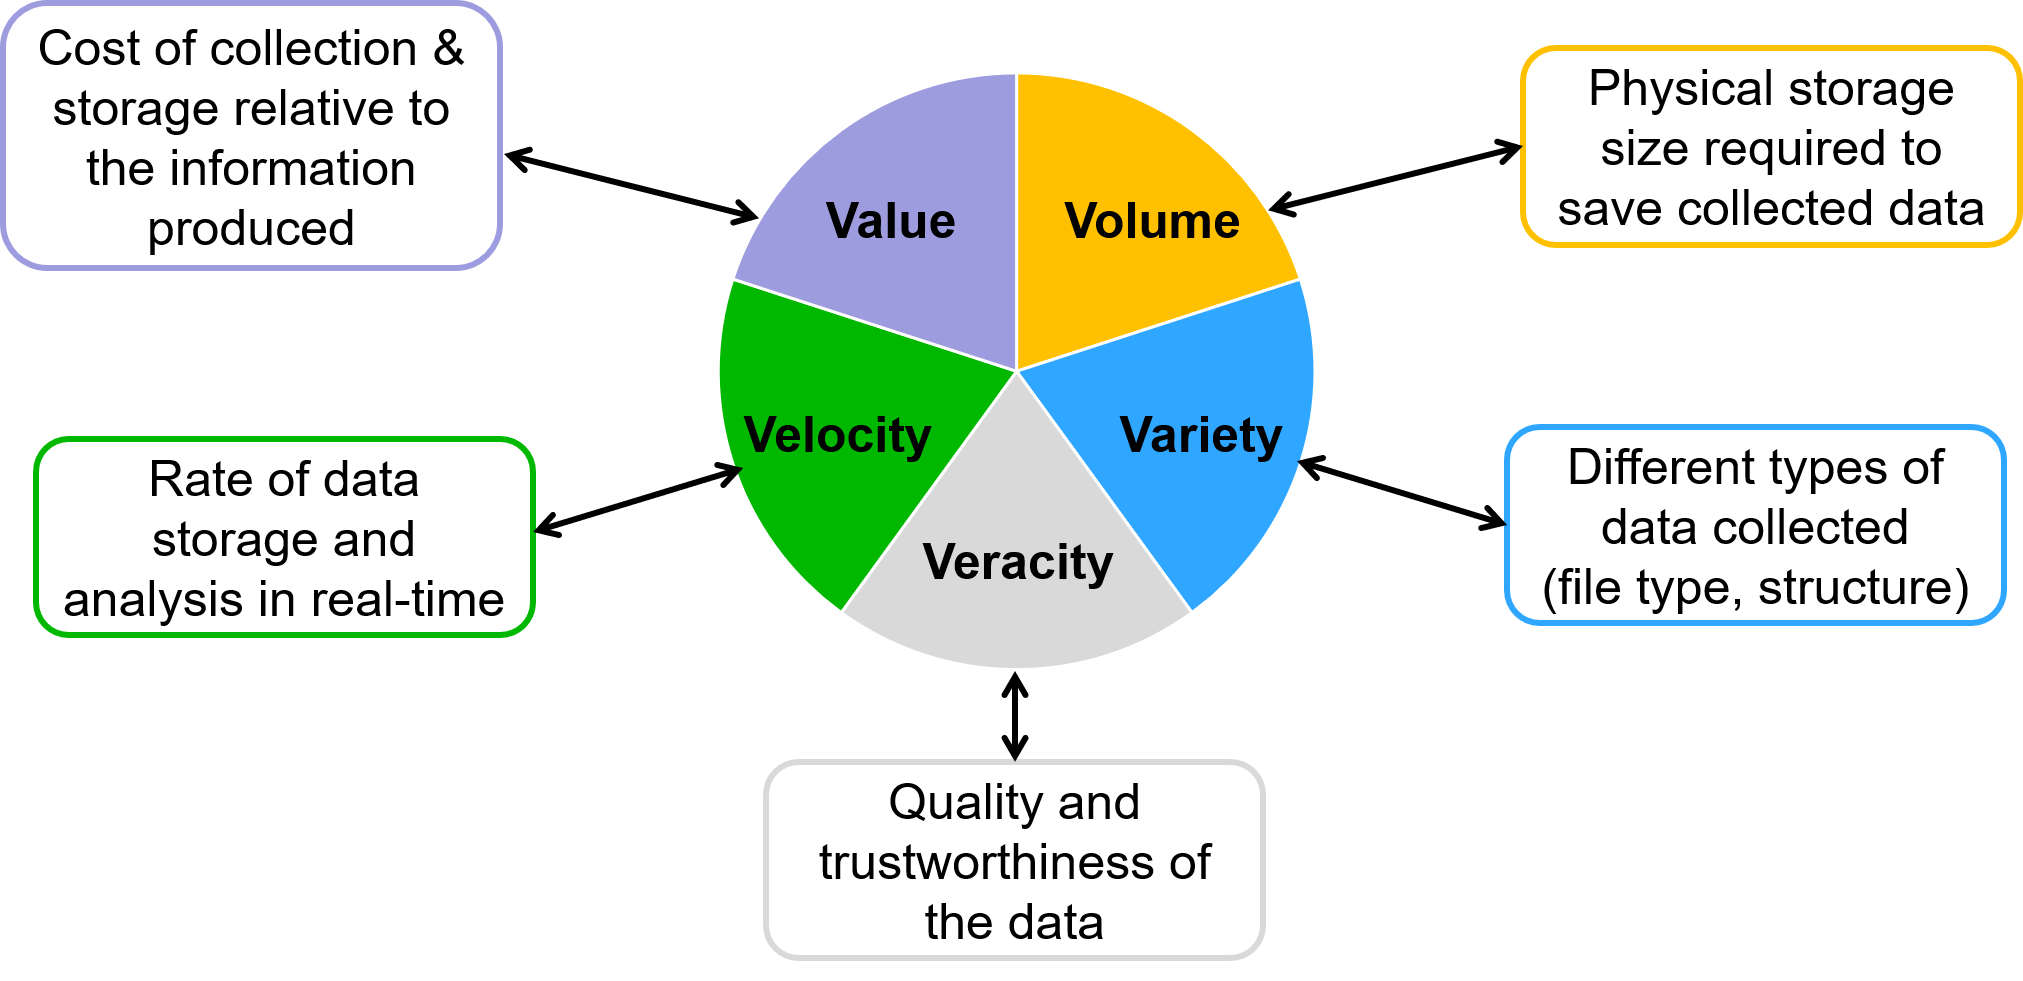
\includegraphics{images/char_big_data.png}

\end{frame}

\begin{frame}{Principal Component Analysis}
\protect\hypertarget{principal-component-analysis}{}

\begin{columns}[T]
\begin{column}{0.48\textwidth}
\begin{itemize}
\tightlist
\item
  Data reduction technique
\item
  Complex relationships between water quality variables

  \begin{itemize}
  \tightlist
  \item
    Interpretable linear combinations of data
  \end{itemize}
\item
  Which components represent the most variability?

  \begin{itemize}
  \tightlist
  \item
    1st component = maximum variance
  \end{itemize}
\end{itemize}
\end{column}

\begin{column}{0.48\textwidth}
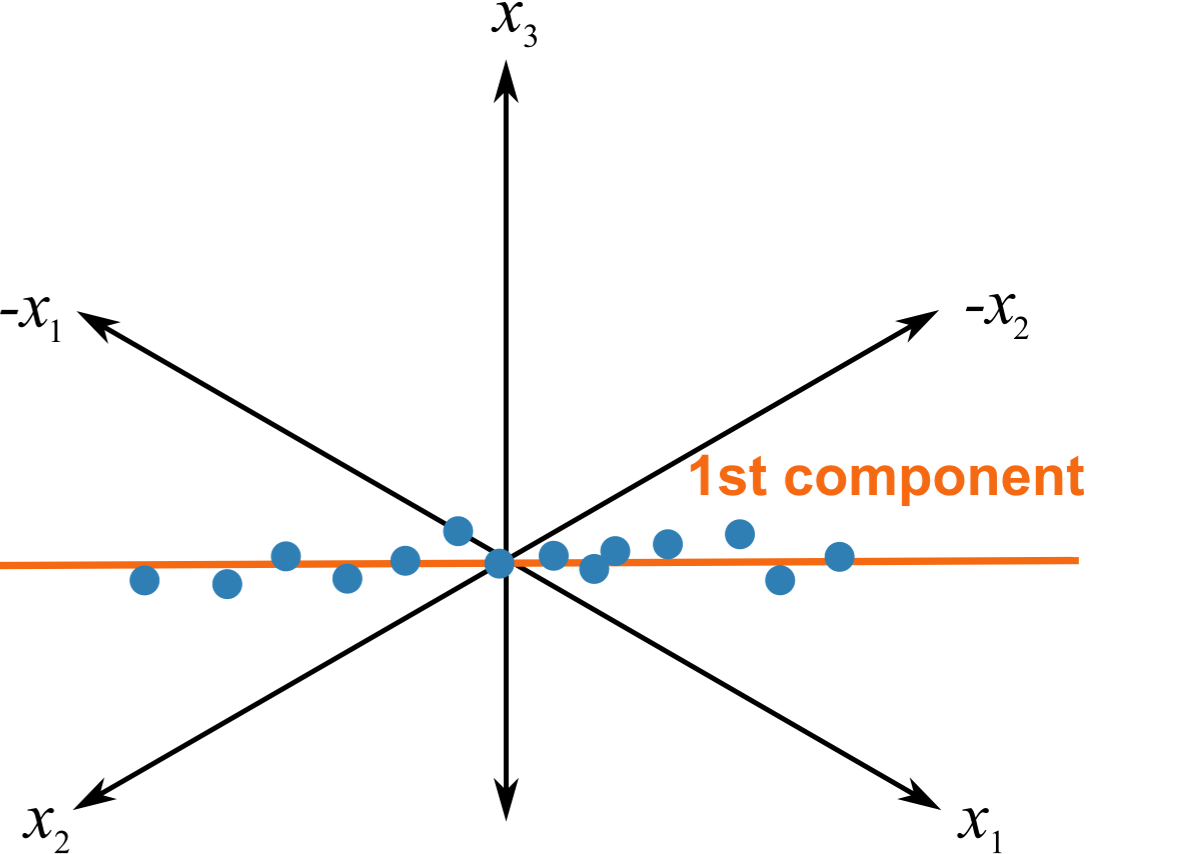
\includegraphics{images/pca.png}
\end{column}
\end{columns}

\end{frame}

\begin{frame}{Mines Park WWTP}
\protect\hypertarget{mines-park-wwtp}{}

\begin{figure}
   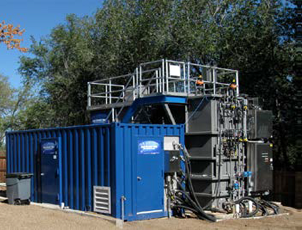
\includegraphics{images/sbmbr.png}
\end{figure}

\end{frame}

\begin{frame}{Mines Park WWTP}
\protect\hypertarget{mines-park-wwtp-1}{}

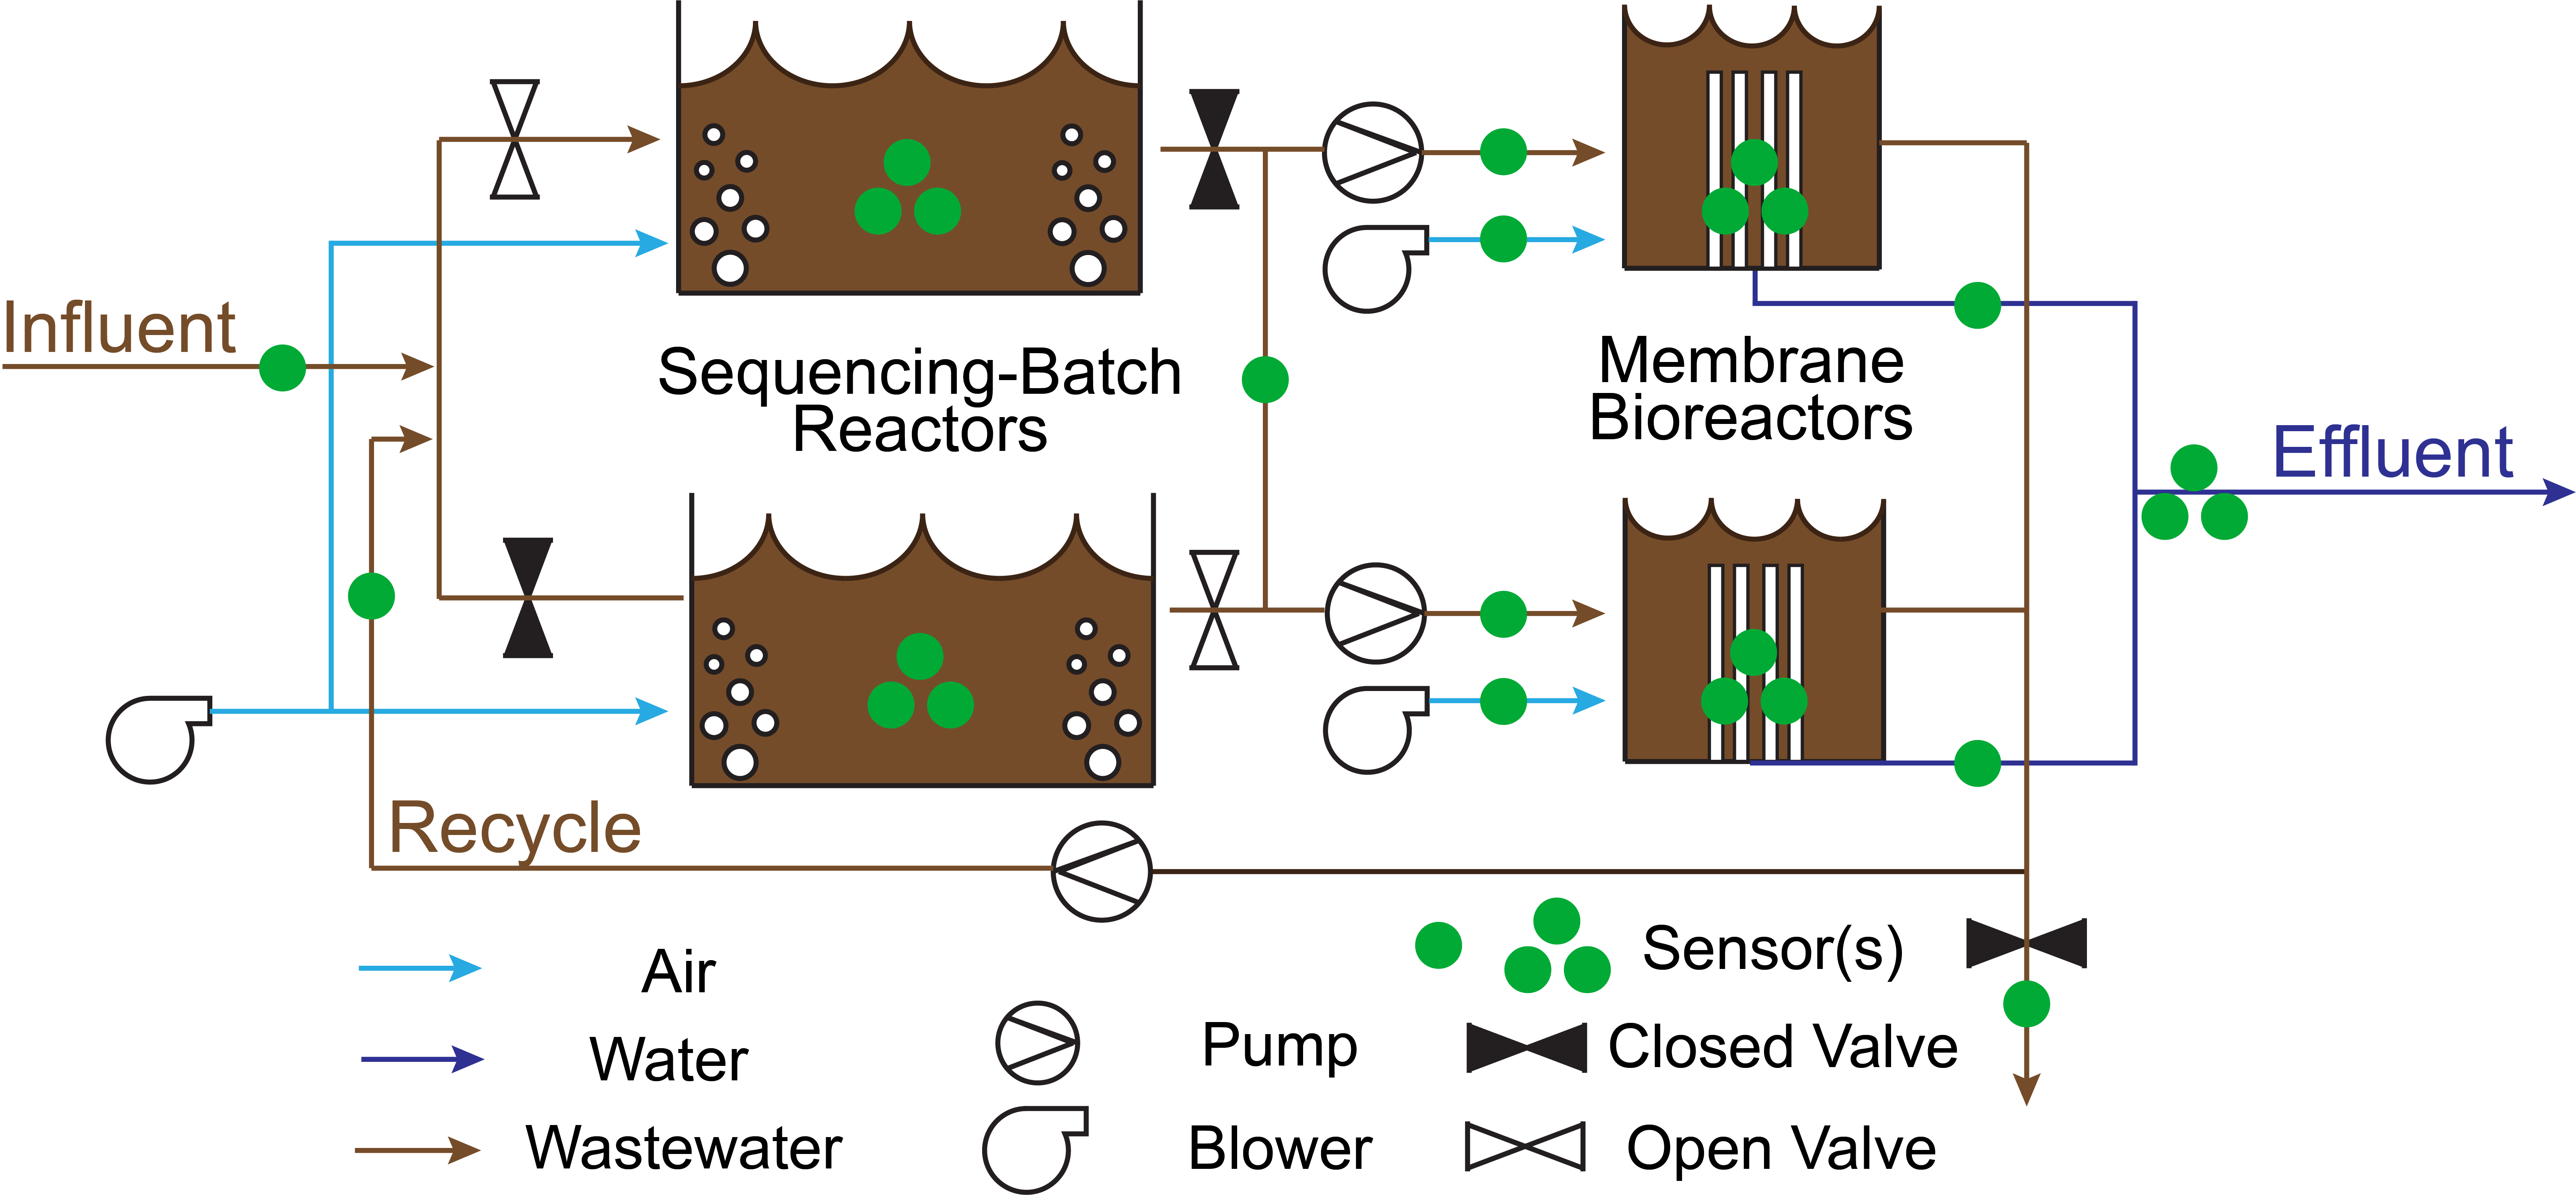
\includegraphics{images/sbmbr_flow_diagram.png}

\end{frame}

\begin{frame}{Case studies}
\protect\hypertarget{case-studies}{}

Steps for each case study:

\begin{enumerate}
\tightlist
\item
  Declare case study parameters
\item
  Compile \& clean raw data
\item
  Train ADPCA model
\item
  Test ADPCA model
\item
  Calculate fault detection statistics
\item
  Summarize results
\end{enumerate}

Required software:

\begin{itemize}
\tightlist
\item
  R (free)
\item
  Student-developed packages (e.g., mvMonitoring, ADPCA)
\end{itemize}

\end{frame}

\begin{frame}{Case study: membrane failure - 7 days}
\protect\hypertarget{case-study-membrane-failure---7-days}{}

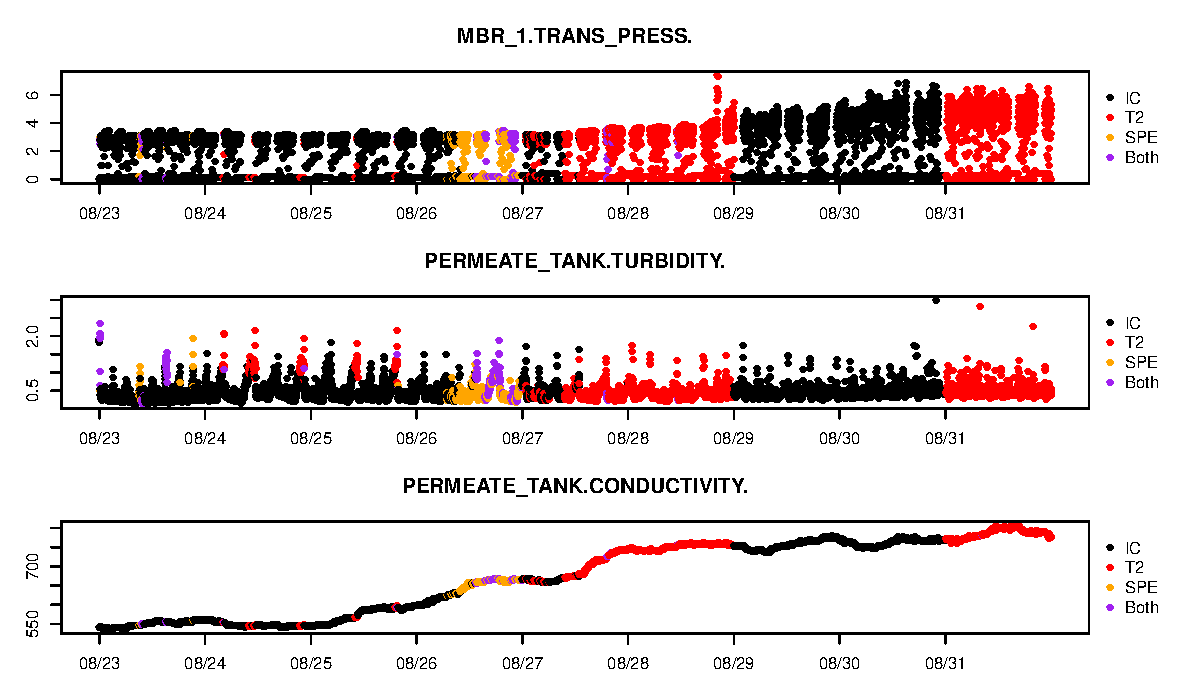
\includegraphics{images/7 day SS allGraphs 2018-08-23 2018-09-01.pdf}

\end{frame}

\begin{frame}{Case study: membrane failure - 5 days}
\protect\hypertarget{case-study-membrane-failure---5-days}{}

\includegraphics{images/5 day SS allGraphs 2018-08-23 2018-09-01.pdf}

\end{frame}

\begin{frame}{Case study: pump shutdown - 10 days - ms}
\protect\hypertarget{case-study-pump-shutdown---10-days---ms}{}

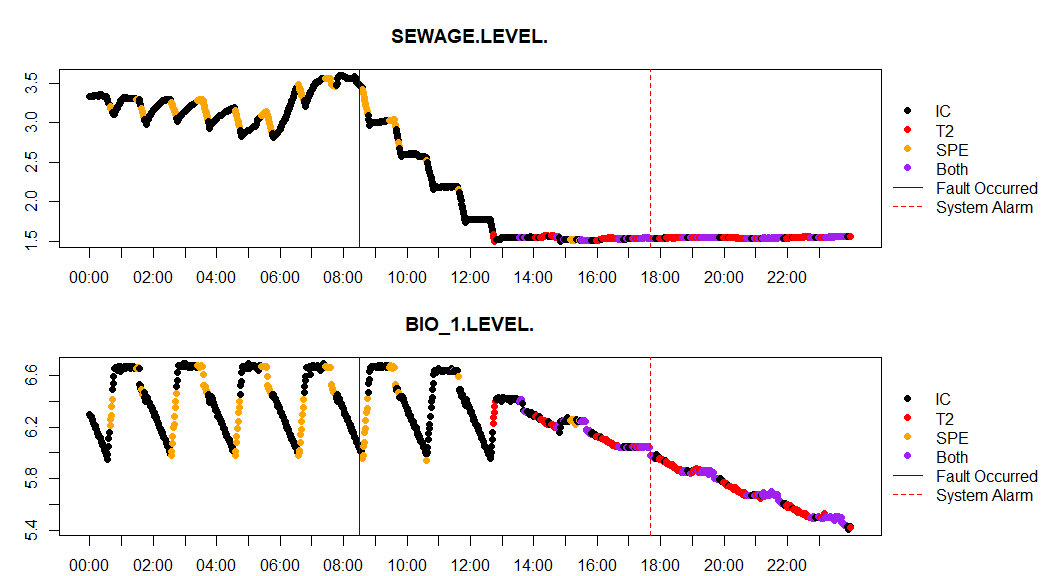
\includegraphics{images/10 day BR allGraphs 2018-01-29 2018-01-30.pdf}

\end{frame}

\begin{frame}{Case study: pump shutdown - 7 days - ms}
\protect\hypertarget{case-study-pump-shutdown---7-days---ms}{}

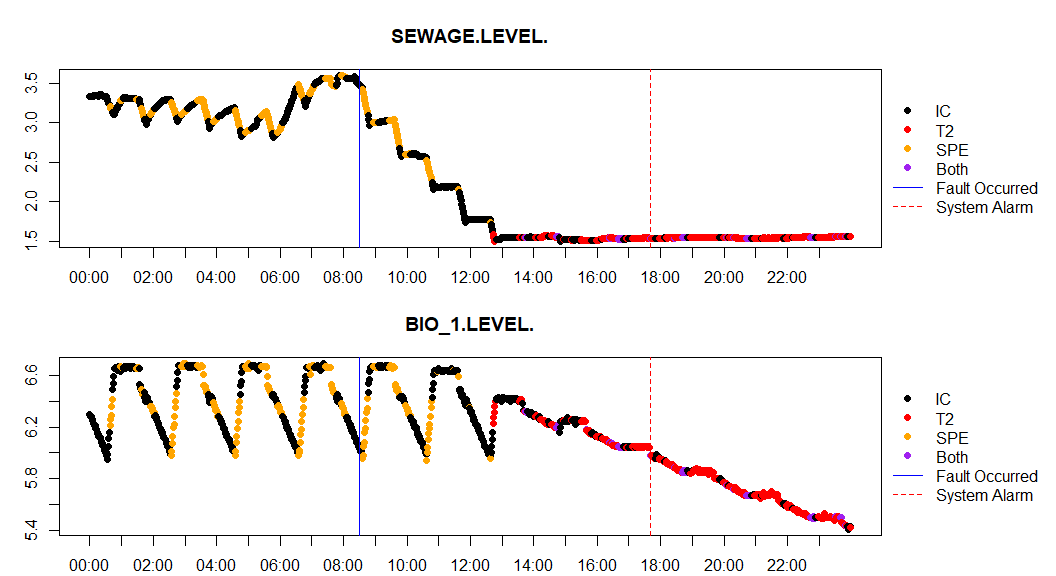
\includegraphics{images/7 day BR allGraphs 2018-01-29 2018-01-30.pdf}

\end{frame}

\begin{frame}{Case study: pump shutdown - 5 days - ms}
\protect\hypertarget{case-study-pump-shutdown---5-days---ms}{}

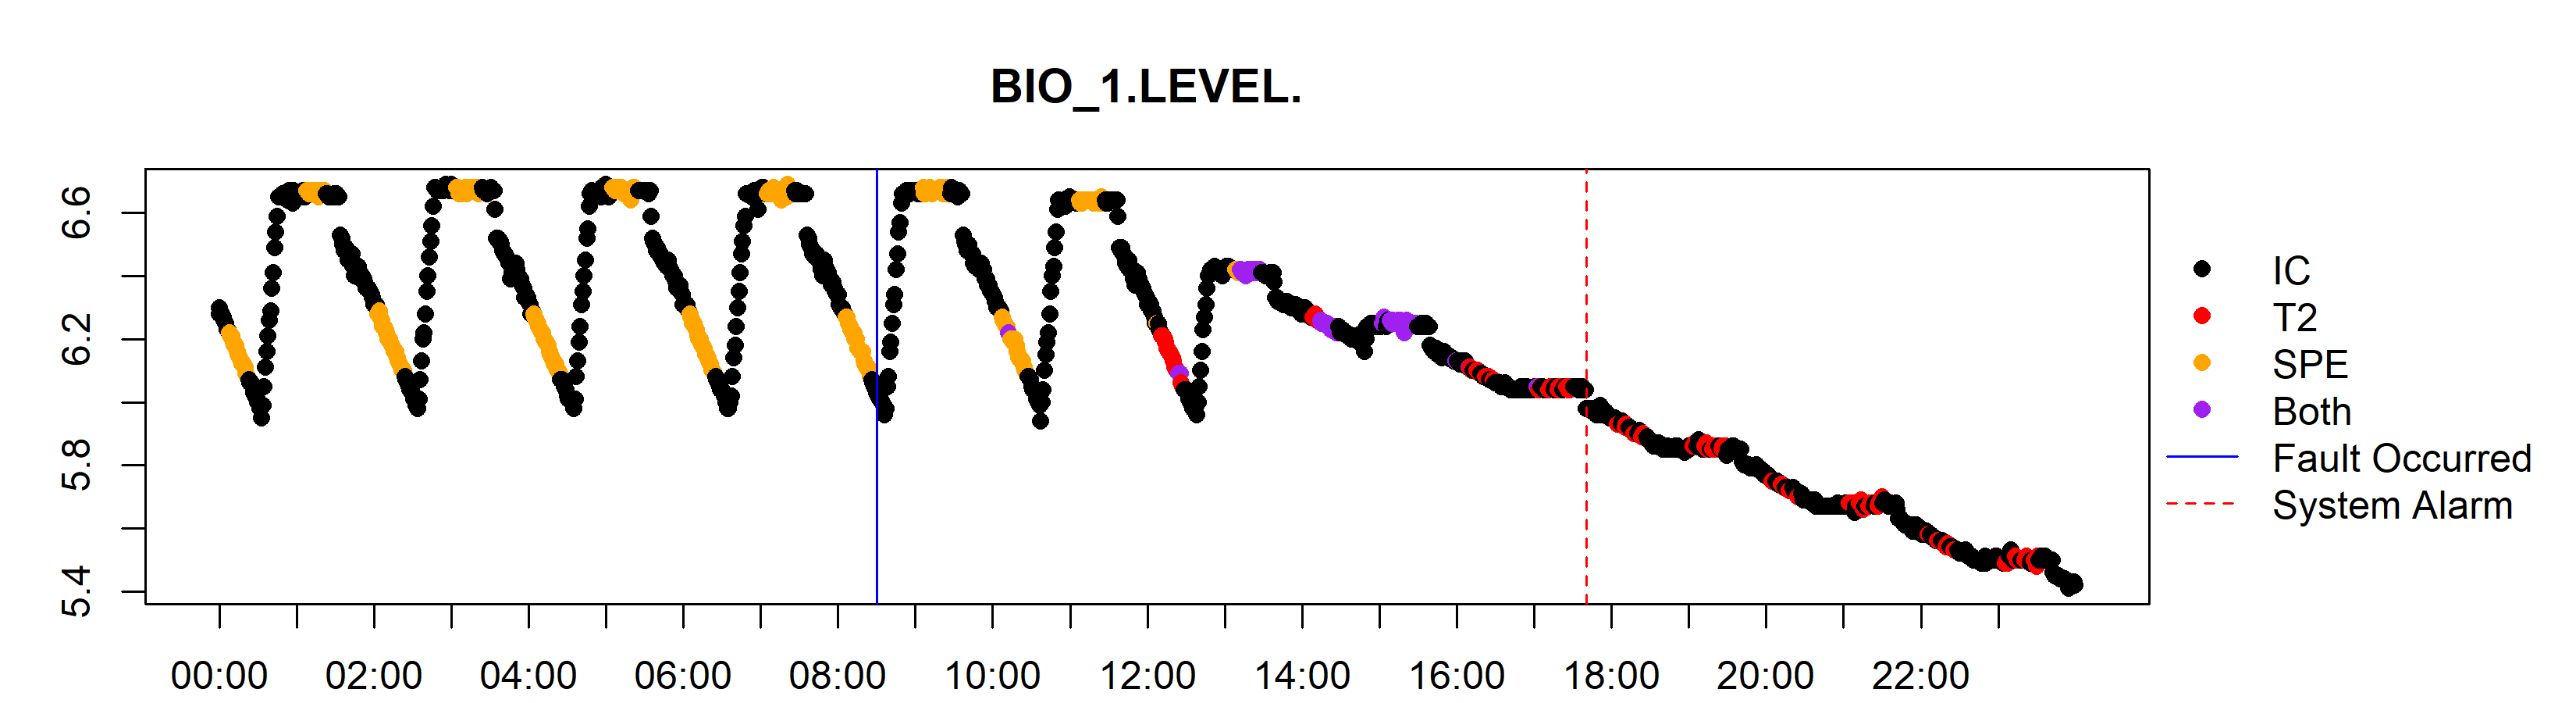
\includegraphics{images/5 day BR allGraphs 2018-01-29 2018-01-30.pdf}

\end{frame}

\begin{frame}{Case study: pump shutdown - 10 days - ss}
\protect\hypertarget{case-study-pump-shutdown---10-days---ss}{}

\includegraphics{images/10 day ss allGraphs 2018-01-29 2018-01-30.pdf}

\end{frame}

\begin{frame}{Case study: pump shutdown - 7 days - ss}
\protect\hypertarget{case-study-pump-shutdown---7-days---ss}{}

\includegraphics{images/7 day ss allGraphs 2018-01-29 2018-01-30.pdf}

\end{frame}

\begin{frame}{Case study: pump shutdown - 5 days - ss}
\protect\hypertarget{case-study-pump-shutdown---5-days---ss}{}

\includegraphics{images/5 day ss allGraphs 2018-01-29 2018-01-30.pdf}

\end{frame}

\begin{frame}{Case study: pump clog - 5 days}
\protect\hypertarget{case-study-pump-clog---5-days}{}

\includegraphics{images/5 day SS allGraphs 2018-01-01 2018-01-25.pdf}

\end{frame}

\begin{frame}{Case study: membrane shutdown - 10 days - ss}
\protect\hypertarget{case-study-membrane-shutdown---10-days---ss}{}

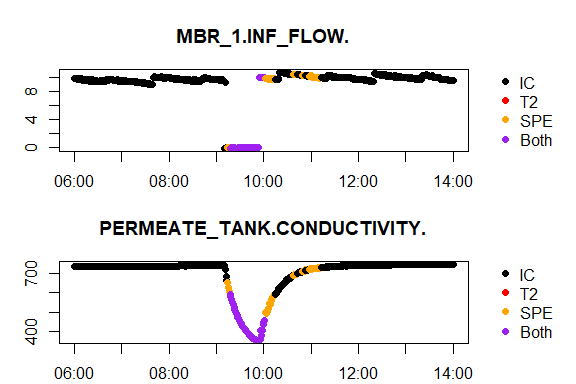
\includegraphics{images/10 day SS allGraphs 2018-01-05 2018-01-05.pdf}

\end{frame}

\begin{frame}{Case study: membrane shutdown - 10 days - ms}
\protect\hypertarget{case-study-membrane-shutdown---10-days---ms}{}

\includegraphics{images/10 day MT allGraphs 2018-01-05 2018-01-05.pdf}

\end{frame}

\begin{frame}{Case study: membrane shutdown - 5 days - ss}
\protect\hypertarget{case-study-membrane-shutdown---5-days---ss}{}

\includegraphics{images/5 day SS allGraphs 2018-01-05 2018-01-05.pdf}

\end{frame}

\begin{frame}{Case study: influent overdose - 5 days}
\protect\hypertarget{case-study-influent-overdose---5-days}{}

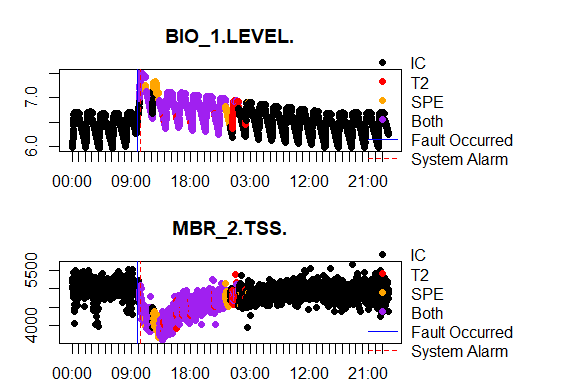
\includegraphics{images/5 day SS allGraphs 2018-01-18 2018-01-20.pdf}

\end{frame}

\begin{frame}{Case study: inf/eff quality changes - 5 days - ss}
\protect\hypertarget{case-study-infeff-quality-changes---5-days---ss}{}

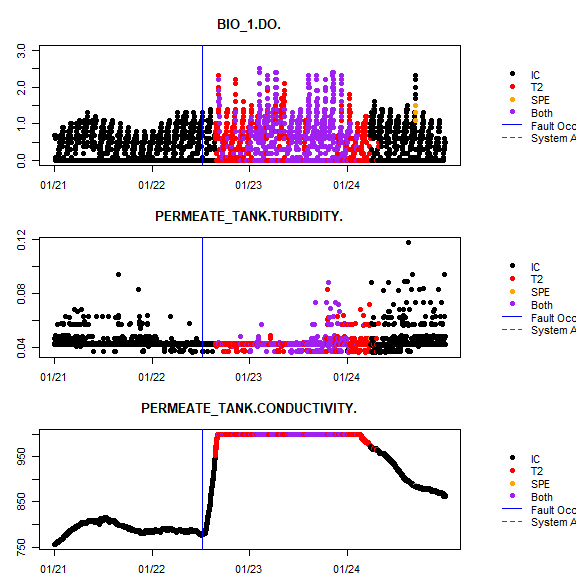
\includegraphics{images/5 day SS allGraphs 2018-01-21 2018-01-25.pdf}

\end{frame}

\begin{frame}{Case study: inf/eff quality changes - 10 days - ss}
\protect\hypertarget{case-study-infeff-quality-changes---10-days---ss}{}

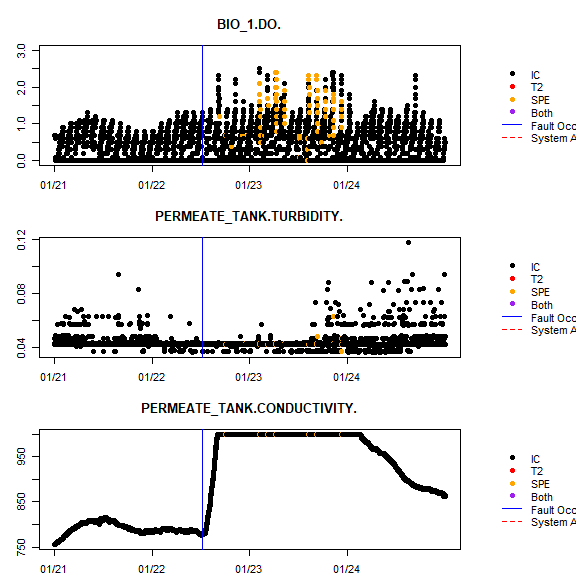
\includegraphics{images/10 day SS allGraphs 2018-01-21 2018-01-25.pdf}

\end{frame}

\begin{frame}{Case study: inf/eff quality changes - 10 days - ms}
\protect\hypertarget{case-study-infeff-quality-changes---10-days---ms}{}

\includegraphics{images/10 day MT allGraphs 2018-01-22 2018-01-24.pdf}

\end{frame}

\begin{frame}{Case study: Clear clog in pump - 5 days - ss}
\protect\hypertarget{case-study-clear-clog-in-pump---5-days---ss}{}

\includegraphics{images/5 day SS allGraphs 2018-01-24 2018-01-29.pdf}

\end{frame}

\begin{frame}{Alarm rates: January - 5 day}
\protect\hypertarget{alarm-rates-january---5-day}{}

\end{frame}

\begin{frame}{Alarm rates: January - 10 day}
\protect\hypertarget{alarm-rates-january---10-day}{}

\end{frame}

\end{document}
